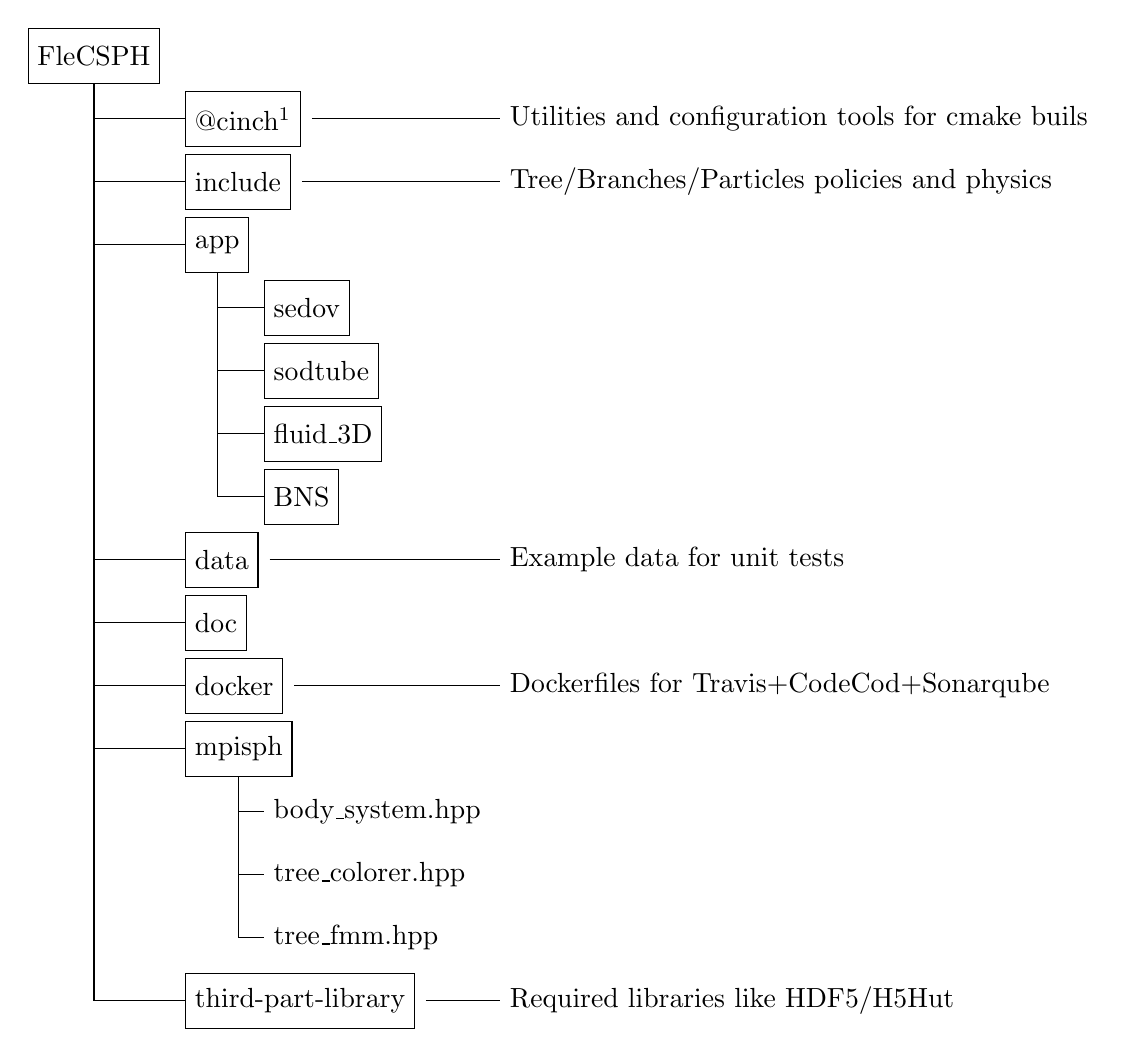
\begin{tikzpicture}
	\def\dist{.8}
	\def\y{10}

	\node[draw,anchor=west,minimum height=.7cm] at (0,\y) (flecsph) {FleCSPH};

	\pgfmathparse{\y-\dist}\edef\y{\pgfmathresult}
	\node[draw,anchor=west,minimum height=.7cm] at (2,\y) (cinch) {@cinch\footnote{https://www.github.com/laristra/cinch}};
	\draw (flecsph.south) |- (cinch.west) -| (cinch.west); 
	\node[anchor=west] at (6,\y) (text) {Utilities and configuration tools for cmake buils};
	\draw ([xshift=4pt]cinch.east) -- ([xshift=-5pt]text);

	\pgfmathparse{\y-\dist}\edef\y{\pgfmathresult}
	\node[draw,anchor=west,minimum height=.7cm] at (2,\y) (include) {include};
	\draw (flecsph.south) |- (include.west) -| (include.west); 
	\node[anchor=west] at (6,\y) (text) {Tree/Branches/Particles policies and physics};
	\draw ([xshift=4pt]include.east) -- ([xshift=-5pt]text);

	\pgfmathparse{\y-\dist}\edef\y{\pgfmathresult}
	\node[draw,anchor=west,minimum height=.7cm] at (2,\y) (app) {app};
	\draw (flecsph.south) |- (app.west) -| (app.west); 
	\pgfmathparse{\y-\dist}\edef\y{\pgfmathresult}
	\node[draw,anchor=west,minimum height=.7cm] at (3,\y) (sedov) {sedov};
	\draw (app.south) |- (sedov.west) -| (sedov.west); 
	\pgfmathparse{\y-\dist}\edef\y{\pgfmathresult}
	\node[draw,anchor=west,minimum height=.7cm] at (3,\y) (sodtube) {sodtube};
	\draw (app.south) |- (sodtube.west) -| (sodtube.west); 
	\pgfmathparse{\y-\dist}\edef\y{\pgfmathresult}
	\node[draw,anchor=west,minimum height=.7cm] at (3,\y) (fluid3D) {fluid\_3D};
	\draw (app.south) |- (fluid3D.west) -| (fluid3D.west); 
	\pgfmathparse{\y-\dist}\edef\y{\pgfmathresult}
	\node[draw,anchor=west,minimum height=.7cm] at (3,\y) (bns) {BNS};
	\draw (app.south) |- (bns.west) -| (bns.west); 

	\pgfmathparse{\y-\dist}\edef\y{\pgfmathresult}
	\node[draw,anchor=west,minimum height=.7cm] at (2,\y) (data) {data};
	\draw (flecsph.south) |- (data.west) -| (data.west);
	\node[anchor=west] at (6,\y) (text) {Example data for unit tests};
	\draw ([xshift=4pt]data.east) -- ([xshift=-5pt]text); 

	\pgfmathparse{\y-\dist}\edef\y{\pgfmathresult}
	\node[draw,anchor=west,minimum height=.7cm] at (2,\y) (doc) {doc};
	\draw (flecsph.south) |- (doc.west) -| (doc.west); 

	\pgfmathparse{\y-\dist}\edef\y{\pgfmathresult}
	\node[draw,anchor=west,minimum height=.7cm] at (2,\y) (docker) {docker};
	\draw (flecsph.south) |- (docker.west) -| (docker.west); 
	\node[anchor=west] at (6,\y) (text) {Dockerfiles for Travis+CodeCod+Sonarqube};
	\draw ([xshift=4pt]docker.east) -- ([xshift=-5pt]text); 

	\pgfmathparse{\y-\dist}\edef\y{\pgfmathresult}
	\node[draw,anchor=west,minimum height=.7cm] at (2,\y) (mpisph) {mpisph};
	\draw (flecsph.south) |- (mpisph.west) -| (mpisph.west); 
	\pgfmathparse{\y-\dist}\edef\y{\pgfmathresult}
	\node[anchor=west,minimum height=.7cm] at (3,\y) (file) {body\_system.hpp};
	\draw (mpisph.south) |- (file.west) -| (file.west); 
	\pgfmathparse{\y-\dist}\edef\y{\pgfmathresult}
	\node[anchor=west,minimum height=.7cm] at (3,\y) (file) {tree\_colorer.hpp};
	\draw (mpisph.south) |- (file.west) -| (file.west); 
	\pgfmathparse{\y-\dist}\edef\y{\pgfmathresult}
	\node[anchor=west,minimum height=.7cm] at (3,\y) (file) {tree\_fmm.hpp};
	\draw (mpisph.south) |- (file.west) -| (file.west); 


	\pgfmathparse{\y-\dist}\edef\y{\pgfmathresult}
	\node[draw,anchor=west,minimum height=.7cm] at (2,\y) (third) {third-part-library};
	\draw (flecsph.south) |- (third.west) -| (third.west); 
	\node[anchor=west] at (6,\y) (text) {Required libraries like HDF5/H5Hut};
	\draw ([xshift=4pt]third.east) -- ([xshift=-5pt]text); 

\end{tikzpicture}